\chapter{The Rebinder}
\label{chap:rebinder}

In the compiler literature, \textit{hoisting} (also known as
\textit{loop-invariant code motion}) is the movement of loop-invariant
expressions out of a loop.  This has a clear benefit: rather than
executing once per iteration of the loop, the expression is executed
once before the loop begins.  For \LO{}, hoisting can be an important
optimisation, as it holds the potential for moving bounds checks and
other assertions out of inner loops.  We will see an example of this
in the next section.

Common Subexpression Elimination (henceforth referred to as CSE) is a
popular compiler optimisation that identifies identical expressions
(i.e. expressions that always evaluate to the same value), and
replaces them with a variable holding the computed value.  If the
common expressions are expensive or computed very frequently, e.g. by
being part of an inner loop, this can result in significant speedup.

It turns out that hoisting and common subexpression elimination can be
unified in a single framework, which in the \LO{} compiler is termed
the \textit{Rebinder}.

This chapter will start out by describing basic principles of hoisting
and CSE in \cref{sec:hoisting,sec:cse}.  In \cref{sec:rebinder}, we
will describe their implementation in the \LO{} compiler.

\section{Hoisting}
\label{sec:hoisting}

When compiling an imperative language,
we must be careful not to move any code with side effects, but in a
pure language such as \LO{}, we can hoist freely (with a few
restrictions that I'll get to in \cref{sec:when-not-to-hoist}).  A
simple example of hoisting in action is shown on
\cref{fig:simple-hoisting}.

\begin{figure}
\begin{center}
\begin{bcolorcode}
map(fn int (int x) =>
      let k = y + z in
      x + k,
    a)
\end{bcolorcode}
\hspace{1cm}
\adjustbox{valign=t}{
\(\Rightarrow\)
}%
\hspace{1cm}
\begin{bcolorcode}
let k = y + z in
map(fn int (int x) =>
      x + k,
    a)
\end{bcolorcode}
\end{center}

\caption{Hoisting in action}
\label{fig:simple-hoisting}
\end{figure}

At first glance, hoisting may seem to apply too rarely to be of much
benefit, since most programmers would put loop-invariant code outside
of the loop in the first place.  However, there are two important use
cases that do not involve programmer-written code:

\begin{itemize}
\item Much \LO{} code is not written by the programmer, but is rather
  the result of program transformation by the compiler.  Inlining and
  constant folding may easily result in the creation of loop-invariant
  expressions within a loop.

\item Explicit bounds checks, as introduced in \cref{sec:assertions},
  can sometimes be hoisted out of inner loops.
\end{itemize}

The latter case merits futher elaboration.  Consider the following
program:

\begin{colorcode}
map(fn int (int i) =>
      a[i] + a[i*2],
    iota(n))
\end{colorcode}

Here, \texttt{a} is a free variable.  Once the compiler has turned the
implicit bound checks explicit, the program will look like this:

\begin{colorcode}
map(fn int (int i) =>
      let c1 = assert(i   >= 0 && i   < size(0,a)) in
      let c2 = assert(i*2 >= 0 && i*2 < size(0,a)) in
      a[<c1>|i] + a[<c2>|i*2],
    iota(n))
\end{colorcode}

Now, the assertions are not loop-invariant, as they depend on
\texttt{i}.  If we assume a sufficiently smart compiler, for example
by employing some extension of \textit{symbolic range
  propagation}\cite{blume1995symbolic}, we can deduce that the
variable \textit{i} will always be in the range $[0,n-1]$.  This
allows us to rewrite the assertions -- the checks for non-negativity
goes away, as it is always true, and we only have to check the upper
bound for the maximum values that \texttt{i} and \texttt{i*2} may
attain:

\begin{colorcode}
map(fn int (int i) =>
      let c1 = assert(n   < size(0,a)) in
      let c2 = assert(n*2 < size(0,a)) in
      a[<c1>|i] + a[<c2>|i*2],
    iota(n))
\end{colorcode}

Now \texttt{c1} and \texttt{c2} are loop-invariant, and we can move
them out of the loop body, and perform bounds checking just once,
before entering the loop:

\begin{colorcode}
let c1 = assert(n   < size(0,a)) in
let c2 = assert(n*2 < size(0,a)) in
map(fn int (int i) =>
      a[<c1>|i] + a[<c2>|i*2],
    iota(n))
\end{colorcode}

For a simple loop such as the above, the potential benefits are great,
as most of the instructions of the original loop body was devoted to
bounds checkings.

The \LO{} compiler does not yet support the range analysis that
enables the critical rewrite of the \texttt{assert} expressions.  An
unpublished bachelors thesis by Jonas Brunsgaard and Rasmus Wriedt
Larsen suggests that the technique works in practice, but their work
has not yet been merged with the main compiler code base.

Hoisting assertions such as these is useful not only when the program
uses explicit array indexing.  While the array accesses performed by
SOACs are by construction always in-bounds, and therefore do not need
dynamic checks, the \texttt{assert} expressions we generate when
transforming from external SOACs to tupleless SOACs are conceptually
identical to bounds checks, and similarly important to hoist.  For
example, consider this program:

\begin{colorcode}
map(fn [int] ([int] r) =>
      map(op+, zip(r, b)),
    a)
\end{colorcode}

After transformation to internal \LO{}, we get the following:

\begin{colorcode}
mapT(fn \{[int]\} ([int] r) =>
       let c = assert(size(0,r) = size(0,b)) in
       <c>mapT(op+, r, b),
    a)
\end{colorcode}

The assertion is not loop-invariant, and range analysis is no help.
For this case, structural size analysis (described in depth in
\cref{sec:size-analysis}) reveals that since \texttt{r} is a row of
\texttt{a}, the outer size of \texttt{r} (\texttt{size(0,r)}) is equal
to the inner size of \texttt{a} (\texttt{size(1,a)}).  Thus, the
compiler rewrites to:

\begin{colorcode}
mapT(fn \{[int]\} ([int] r) =>
       let c = assert(size(1,a) = size(0,b)) in
       <c>mapT(op+, r, b),
    a)
\end{colorcode}

The assertion is now loop-invariant and can be hoisted:

\begin{colorcode}
let c = assert(size(1,a) = size(0,b)) in
mapT(fn \{[int]\} ([int] r) =>
       <c>mapT(op+, r, b),
    a)
\end{colorcode}

The details of how hoisting is implemented in the \LO{} compiler is
covered in \cref{sec:rebinder}.

\subsection{What not to hoist}
\label{sec:when-not-to-hoist}

Clearly, we can hoist only loop-invariant expressions.  Unfortunately,
not all loop-invariant expressions are hoistable, and as is often the
case when seemingly valid transformations become problematic,
constraints imposed by uniqueness types are at fault.  Consider the
following program:

\begin{colorcode}
map(fn (int i) =>
      let a = iota(10) in
      f(a, i),
    b)
\end{colorcode}

It seems that we should be able to hoist \texttt{a} out of the loop
like this:

\begin{colorcode}
let a = iota(10) in
map(fn (int i) =>
      f(a, i),
    b)
\end{colorcode}

However, if the function call \texttt{f(a,i)} consumes the \texttt{a}
argument, hoisting would result in an invalid program, as \texttt{a}
would be consumed multiple times.  We need a ``freshly allocated''
\texttt{a} for each iteration of the loop.  Hence, we must not hoist a
binding out of a loop in which it is consumed.

As a minor, but important point, it is strictly not permitted to hoist
out of loops unless it can be proven that the loop will always execute
at least one iteration.  The \LO{} compiler currently ignores this
restriction, implicitly assuming that all arrays are non-empty.

\subsubsection{Hoisting out of branches}

Most compilers generally do not hoist out of branches, as branching is
often used to prevent expensive execution of expensive expressions
whose value is not needed.  On many GPUs however, execution happens in
lock-step across all processors.  This implies that unless the branch
condition computes the same value in all threads, both sides of the
branch will have to be executed~\cite{reducing-branch-divergence}.
This implies that in some cases, hoisting out of a branch does not
cause more instructions to be executed, and hoisting might expose the
possibility of other optimisations, particularly common subexpression
elimination (see \cref{sec:cse}).

We should still be careful when hoisting expressions out of the
branches of a conditional, as it is possible that the expression may
result in an error unless the condition checked by the conditional is
true.  For example, consider this expression:

\begin{colorcode}
if \(c\) then y / x
     else if \(p\) then y / x
               else 0
\end{colorcode}

If \texttt{y / x} was hoisted out of the branch, the resulting program
might end up dividing by zero.  Assertions and array indexing are
other operations that are not safe to hoist out of a branch.  Most
expressions are safe however, and the \LO{} compiler aggressively
hoists these out of branches.  Depending on improvements in hardware,
or the targeting of \LO{} for non-GPU systems, it is likely that this
strategy will need to be revised.

\subsubsection{Performance Considerations}

There is another potential case where hoisting, while not resulting in
an invalid program, proves detrimental rather than beneficial to
performance.  This occurs when retrieving the hoisted value from
memory would be more expensive than re-computing it for each loop
iteration, which is particularly likely to occur on GPUs, as global
memory accesses are enormously expensive.  Balancing this problem is
not currently tackled by the \LO{} compiler, which instead hoists as
aggressively as possible.  Note that this is not a problem when
hoisting assertions, such as bounds checks, as the resulting values
are not actually accessed from within the loop.

\section{Common Subexpression Elimination}
\label{sec:cse}

Common Subexpression Elimination (henceforth referred to as CSE) is a
popular compiler optimisation that identifies identical expressions
(i.e. expressions that always evaluate to the same value), and
replaces them with a variable holding the value.  For example, this
program:

\begin{colorcode}
2 * x + 2 * x
\end{colorcode}

Can be transformed through CSE into:

\begin{colorcode}
let tmp = 2 * x in
tmp + tmp
\end{colorcode}

This saves us a multiplication.  As with hoisting, CSE can potentially
be detrimental to performance if it increases memory pressure, but
again like hoisting, this is not something the \LO{} compiler
currently takes into consideration.

We must be careful not to perform CSE such that we end with a
violation of the uniqueness rules.  Consider this program:

\begin{colorcode}
let a = iota(10) in
let b = iota(10) in
let a[2] = 5 in
f(a,b)
\end{colorcode}

Since \texttt{iota(10)} appears in two places, we might be tempted to
factor it out:

\begin{colorcode}
let tmp = iota(10) in
let a = tmp in
let b = tmp in
let a[2] = 5 in
f(a,b)
\end{colorcode}

However, this violates Uniqueness Rule 1, as \texttt{b} is aliased to
\texttt{a}, yet is used after \texttt{a} is consumed in a
\texttt{let-with} expression.  The solution is to not perform CSE on
expressions whose result is eventually consumed -- or more
conservatively, never perform CSE on an expression of type
\texttt{*[$\alpha$]}.  The latter is easier to implement, although too
conservative, but is what the \LO{} compiler currently does.

\section{Rebinder Implementation}
\label{sec:rebinder}

Conceptually, hoisting and CSE are rather different transformations.
However, they both depend on identifying subexpressions that can be
moved (in the case of hoisting) or replaced (in the case of CSE), but
where the actual expression rewriting is quite simple.  In the \LO{}
compiler, the observation was made that a lot of the machinery used to
implement hoisting could be easily extended to also perform CSE, and
thus was born a compiler pass with the rather idiosyncratic name
\textit{the Rebinder}.

The central idea is to assume a program in a slightly modified
A-normal form~\cite{Sabry:1992:RPC:141478.141563}, a format similar to
\textit{three address code}, where the definition of each
\texttt{let}-binding is a \textit{simple expression}, and the body of
a \texttt{let}-binding is either another binding or a variable.  A
simple expression is either a branch\footnote{Not permitted in
  ``standard'' A-normal form.}, or an expression where all
subexpressions are variables or constants (except for the bodies of
SOAC functions), which implies that their execution terminates
immediately.  For example, the following program:

\begin{colorcode}
fun real solve(real a, real b, real c) =
  (-b + sqrt(b*b - 4.0*a*c)) / (2.0*a)
\end{colorcode}

Would look like this in A-normal form.  Note that it is also
\texttt{let}-normalised (\cref{sec:let-normalisation}):

\begin{colorcode}
fun real solve(real a_0, real b_1, real c_2) =
  let negate_3  = -b_1 in
  let times_4   = b_1 * b_1 in
  let times_5   = 4.0 * a_0 in
  let times_6   = times_5 * c_2 in
  let minus_7   = times_4 - times_6 in
  let norm_8    = sqrt(minus_7) in
  let plus_9    = negate_3 + norm_8 in
  let times_10  = 2.0 * a_0 in
  let divide_11 = plus_9 / times_10 in
  divide_11
\end{colorcode}

This simplifies hoisting and CSE significantly, as the problem is now
reduced to moving nodes in the syntax tree (for hoisting) and
substituting definitions of \texttt{let}-bindings (for CSE).
A-normalisation is performed by a separate pass before entering the
Rebinder, and is generally trivial, but there are a few difficulties
that I will cover in \cref{sec:simplification-of-expressions}.

In order to keep the exposition simpler, \texttt{loop} and
\texttt{let-with} will be ignored (except with respect to upholding
uniqueness constraints), and only discuss hoisting of normal
\texttt{let}-bindings.

To try to give an intuition of the Rebinder, let us consider the
following contrived program:

\begin{colorcode}
fun int main([int] a, int i, int v) =
  let {res} =
    reduceT(fn \{int\} (int sum, int x) =>
              {sum + x + v*a[i]},
            \{v*a[i]\}, a) in
  res
\end{colorcode}

The goal is to hoist the loop-invariant expression \texttt{v*a[i]} out
of the loop, and use CSE to combine it with the initial value of the
accumulator.  To this end, it is first transformed to A-normal form:

\begin{colorcode}
fun int main([int] a_0, int i_1, int v_2) =
  let index_10 = a_0[i_1] in
  let times_11 = v_2 * index_10 in
  let \{res_5\} =
    reduceT(fn \{int\} (int sum_3, int x_4) =>
              let plus_6 = sum_3 + x_4 in
              let index_7 = a_0[i_1] in
              let times_8 = v_2 * index_7 in
              let plus_9 = plus_6 + times_8 in
              {plus_9},
            \{times_11\}, a_0) in
  res_5
\end{colorcode}

The intuition we will use is to strip an expression $e$ of any
enclosing bindings, resulting in a ``core'' expression $e'$, and a set
of bindings.  There may be free variables in $e'$ that are bound by
the bindings in the set.  At some point, we will have to insert the
bindings in the program, but we will try to put them as far up the
syntax tree as possible.  For example, stripping the body of
\texttt{main} above would result in the core expression
\texttt{res\_5} and the bindings \texttt{index\_10},
\texttt{times\_11}, and \texttt{res\_5}.

The set of bindings, which we will term the \textit{potentially
  hoistable set}, is a partially ordered set of binding pairs
$(p_{i},e_{i})$.  A binding pair $(p_{i},e_{i})$ corresponds to the
\LO{} binding \texttt{let~$p_{i}$~=$e_{i}$}.  The partial order is
$\preceq$: for two bindings $b_{i}, b_{j}$, $b_{i} \preceq b_{j}$ if
$b_{j}$ uses any variables bound by $b_{i}$, or if $b_{i} = b_{j}$.
The potentially hoistable set thus represents an acyclic
data-dependency graph.

The Rebinder proceeds with a recursive walk down the syntax tree,
collecting bindings into the potentially hoistable set.  Additionally,
for each binding, we recurse down its right-hand side in order to
determine whether it contains any \textit{hoistable subexpressions}.
This is only the case if the RHS is a SOAC -- where we can hoist out
of the body -- or \texttt{if} -- where we can hoist out of the
branches.  For all other expressions, due to the program being in
A-normal form, the subexpressions will be variables or constants,
which are not hoisted.

A traversal of the example program listed above follows:

\begin{itemize}
\item First, we encounter the \texttt{index\_10} and
  \texttt{times\_11} bindings, and their right-hand sides are
  inspected.  Neither of these inspections yield hoistable
  subexpressions, but we remove \texttt{index\_10} and
  \texttt{index\_11} themselves and insert them into the potentially
  hoistable set.

\item Next, we encounter the \texttt{res\_5} binding and we descend
  recursively into the scope of the SOAC function body:

  \begin{itemize}
  \item We inspect the right-hand sides of \texttt{plus\_6},
    \texttt{index\_7}, \texttt{times\_8} and \texttt{plus\_9}, none of
    which yield hoistable subexpressions.  We collect these bindings
    into a potentially hoistable set and remove them from the function
    body, leaving just the expression \texttt{\{plus\}}.

  \item We are now done inspecting the function, and we need to decide
    which of the bindings in the potentially hoistable set can in fact
    be hoisted out.  The function parameters are \texttt{sum\_3} and
    \texttt{x\_4}, and any bindings that depend on these cannot be
    hoisted (the details are given in \cref{sec:hoisting-bindings}).
    This leaves the bindings for \texttt{index\_7} and
    \texttt{times\_8} as hoistable; while \texttt{plus\_6} and
    \texttt{plus\_9} are re-inserted into the program.
  \end{itemize}

  This yields the \texttt{index\_7} and \texttt{times\_8} bindings as
  new elements in the potentially hoistable set.  We also add the
  modified \texttt{res\_5} binding itself.

\item Since there are no more bindings left, and we are at the top
  level of a function, we insert the bindings in the potentially
  hoistable set (\texttt{index\_10}, \texttt{times\_11},
  \texttt{res\_5}, \texttt{index\_7} and \texttt{times\_8}) in the
  program, yielding:

\begin{colorcode}
fun int main([int] a_0, int i_1, int v_2) =
  let index_10 = a_0[i_1] in
  let times_11 = v_2 * index_10 in
  let index_7 = a_0[i_1] in
  let times_8 = v_2 * index_7 in
  let {res_5} =
    reduceT(fn \{int\} (int sum_3, int x_4) =>
              let plus_6 = sum_3 + x_4 in
              let plus_9 = plus_6 + times_8 in
              \{plus_9\},
            \{times_11\}, a_0) in
  res_5
\end{colorcode}
\end{itemize}

We could now do a separate CSE pass over the entire program, but there
may be a more efficient strategy.  The Rebinder is able to perform the
CSE optimisation whenever we insert the non-hoistable bindings into
the syntax tree.  We will try to provide an intuition for the
approach, using the above example:

When, at the end, we have to insert bindings for \texttt{index\_10},
\texttt{times\_11}, \texttt{res\_5}, \texttt{index\_7} and
\texttt{times\_8}, we have to determine an order that does not result
in a variable being used before it is defined.  This is easy, since
the potentially hoistable set is already dependency-ordered and thus
defines a data dependency graph (shown on
\cref{fig:rebinder-example-graph}).  The following insertion order is
obtained by performing a depth-first traversal of the graph:

\begin{enumerate}
\item \texttt{index\_10}
\item \texttt{times\_11}
\item \texttt{index\_7}
\item \texttt{times\_8}
\item \texttt{res\_5}.
\end{enumerate}

\begin{figure}
\centering
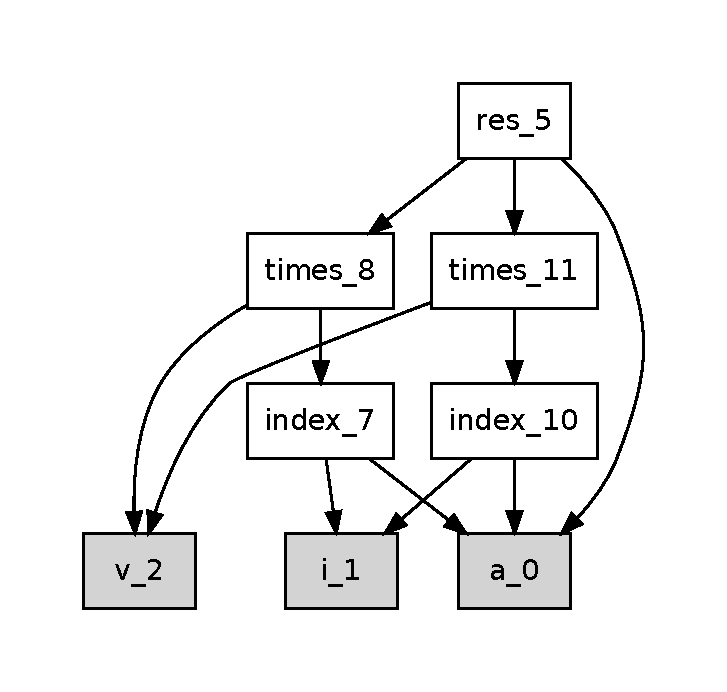
\includegraphics[width=4.5cm]{img/rebinder-ddg.pdf}
\caption{Data dependency graph for example program}
\label{fig:rebinder-example-graph}
\end{figure}

None of these bindings can be removed, as the names they bind may be
used in subexpressions, but their right-hand sides (RHS) can be
changed freely.  This is what is exploited to perform CSE.  The
following steps are performed:

\begin{description}
\item[\texttt{index\_10}:] Inserted unchanged, but we record its RHS,
  in case we end up seeing an identical expression later on.
\item[\texttt{times\_11}:] Likewise inserted unchanged, as its RHS
  does not correspond to any previously seen.
\item[\texttt{index\_7}:] Since the RHS of this binding is identical
  to the RHS of \texttt{index\_10}, we replace the RHS of
  \texttt{index\_7} with the variable \texttt{index\_10}.  We insert
  the resulting binding \texttt{let~times\_11~=~index\_7} and record
  the substitution $\texttt{index\_y}\rightarrow\texttt{index\_10}$.
\item[\texttt{times\_8}:] The substitution
  $\texttt{index\_y}\rightarrow\texttt{index\_10}$ is performed on the
  immediate subexpressions of the RHS, obtaining
  \texttt{v\_2~*~index\_10}, then check whether the resulting
  expression has been seen before.  This turns out to be identical to
  the RHS of \texttt{times\_11}, and therefore we insert the binding
  \texttt{let~times\_8~=~times\_11}.
\item[\texttt{res\_5}:] The substitution
  $\texttt{index\_y}\rightarrow\texttt{index\_10},\texttt{times\_8}\rightarrow\texttt{times\_11}$
  is performed, although no changes are made.  The binding is then
  inserted.
\end{description}

The result is the following program:

\begin{colorcode}
fun int main([int] a_0, int i_1, int v_2) =
  let index_10 = a_0[i_1] in
  let times_11 = v_2 * index_10 in
  let index_7 = index_10 in
  let times_8 = times_11 in
  let {res_5} =
    reduceT(fn \{int\} (int sum_3, int x_4) =>
              let plus_6 = sum_3 + x_4 in
              let plus_9 = plus_6 + times_8 in
              \{plus_9\},
            \{times_11\}, a_0) in
  res_5
\end{colorcode}

Copy propagation can then be used to remove the \texttt{index\_7} and
\texttt{times\_8} bindings.\fixme{This is still way too vague and hard to understand.}

\subsection{Hoisting Bindings}
\label{sec:hoisting-bindings}

The problem is as follows: We are given a potentially hoistable set,
$\{(p_{i}, e_{i})\}$, of patterns $p_{i}$ and $e_{i}$.  Each pattern
$p_{i}$ defines several names that may be used by other expressions in
the set.

We need to split the potentially hoistable set into a
\textit{hoistable set}, and a set of the bindings that cannot be
hoisted further, the \textit{unhoistable set}.  To this end, we are
given a unary relation $\mathcal{B}$, that given a binding $(p_{i},
e_{i})$, tells us whether $e_{i}$ is blocked from being hoisted.  As
the most archetypical reason, $\mathcal{B}(p_{i}, e_{i})$ whenever
$e_{i}$ uses a parameter of the function that we are trying to hoist
out of, but the relation also checks the other cases mentioned in
\cref{sec:when-not-to-hoist}.  We will consider as unhoistable any
binding that is unhoistable according to $\mathcal{B}$, as well as any
binding that depends on an unhoistable binding.

Each of the expressions $e_{i}$ may use variables from any of the
patterns $p_{j}$ (except its own), but there may also be free
variables that are not contained in any pattern in the potentially
hoistable set.  These correspond to names bound higher up in the
program.

Since the potentially hoistable set is partially ordered, we can
process its elements in dependency order.  We keep track of the names
bound by unhoistable bindings in an \textit{unhoisted name set},
initially empty.  For each binding $(p_{i},e_{i})$, we check whether
$\mathcal{B}(p_{i},e_{i})$ or $e_{i}$ uses a name in the unhoisted
name set:
\begin{itemize}
\item If so, the binding is put into the unhoistable set, and the
  names in $p_{i}$ are added to the unhoisted name set.
\item Otherwise, the binding is put into the hoistable set.
\end{itemize}
The end result is a set of hoistable bindings, and a set of
nonhoistable bindings.  Because of the ordering, we are guaranteed
that no binding in the former uses a name bound in the
latter.

\subsection{Inserting Bindings}

After dividing the potentially hoistable set into hoistable and
non-hoistable bindings, we have to insert all non-hoistable bindings
around the core expression.  Concretely, we are given a core
expression $e_{c}$ and an ordered set of expressions
$\{(p_{i},~e_{i})\}$, where binding $(p_{i},~e_{i})$ must precede
binding $(p_{i+1},~e_{i+1})$.  We can take this opportunity to perform
dead code elimination by removing any binding $(p_{i},~e_{i})$ that is
not used in either $e_{c}$ or any enclosed binding.  The idea is to
track which names are actually used in the lexical scope of the
binding, and remove bindings that are never referenced.

The algorithm is as follows.  We will track two pieces of data: A set
$\mathcal{F}$, which is initialised to the free variables of $e_{c}$
\footnote{This can be done efficiently if the rebinder constantly
  tracks the free variables of the core expression.}.  Then we proceed
\textit{backwards} through the list of bindings, i.e., we first
process the binding that should be innermost.  For each binding
$(p_{i},~e_{i})$, we check whether any of the names bound by $p_{i}$
are present in $\mathcal{F}$.  If so, we add the free variables of
$e_{i}$ to $\mathcal{F}$ and insert the binding.  If the binding is
not used, we skip it.

\subsection{Simplification of Expressions}
\label{sec:simplification-of-expressions}

The CSE technique described in the previous sections depends heavily
on semantically identical code also having ($\alpha$-)equivalent
bindings.  However, in many cases, two expressions may have different
syntax trees, yet semantically be the same.  For example, consider the
expressions \texttt{(x*y)*z} versus \texttt{x*(y*z)}.  If we assume
that \texttt{*} is associative\footnote{Strictly not the case for
  floating-point multiplication.}, these expressions will always
compute the same value.  With respect to A-normal form, the two
different normalised expressions are shown on
\cref{fig:differing-normalisation}.

\begin{figure}
\begin{subfigure}[t]{.33\textwidth}
\centering
\begin{colorcode}
let a = x * y in
let b = a * z in
b
\end{colorcode}
\subcaption{\texttt{(x * y) * z}}
\end{subfigure}%
\begin{subfigure}[t]{.33\textwidth}
\centering
\begin{colorcode}
let a = y * z in
let b * x * a in
b
\end{colorcode}
\subcaption{\texttt{x * (y * z)}}
\end{subfigure}%
\begin{subfigure}[t]{.33\textwidth}
\centering
\begin{colorcode}
let a = z * y in
let b * x * a in
b
\end{colorcode}
\subcaption{\texttt{x * (z * y)}}
\end{subfigure}
\caption{Normalisation of syntactically different expressions}
\label{fig:differing-normalisation}
\end{figure}

Despite the syntactical difference between these two expressions, they
are clearly semantically identical, and we would like for CSE to
remove one of them.  Given the way our CSE optimisation works, the
only solution is to ensure that equivalent expessions A-normalise to
$\alpha$-equivalent bindings.  In general, this is a very hard-problem
- in fact, determining whether two expressions will always evaluate to
the same result is undecideable, as it reduces to the halting problem.
Fortunately, the problem becomes quite tractable with restricted to
arithmetic operations, through the use of \textit{simplification}
before employing the normaliser.

One solution, which was implemented in an unpublished bachelors thesis
by Jonas Brunsgaard and Rasmus Wriedt Larsen, is to simplify
arithmetic expressions into a form known as \textit{sum-of-products}.
In this form, the top node of the syntax tree for an arithmetic
expression is always an addition node with $n$ multiplication
children.  Each of these multiplication nodes may have $m$ children,
which can be arbitary numeric expressions.  By ordering the children
of each node according to some criterion (say, lexicographically), we
obtain a unique tree structure for arithmetic expressions that ignores
superficial syntactical differences, such as one shown on
\cref{fig:differing-normalisation}.  This unique tree structure can
then be A-normalised into an equally unique set of bindings.

%%% Local Variables: 
%%% mode: latex
%%% TeX-master: "thesis.tex"
%%% End: 
